We have developed a prototype of our query rewriting algorithm which takes into consideration users' requirements and services' quality aspects extracted from SLAs. The \textit{Rhone} prototype is implemented in Java.

Currently, our approach runs in a local controlled environment simulating a mono-cloud including a service registry of 100 concrete services. 
Experiments were produced to analyze the algorithm's behavior concerning performance, and quality and cost of the integration. The figures~\ref{fig01} and \ref{fig02} summarize our first results.

\begin{figure}[!h]
\centering
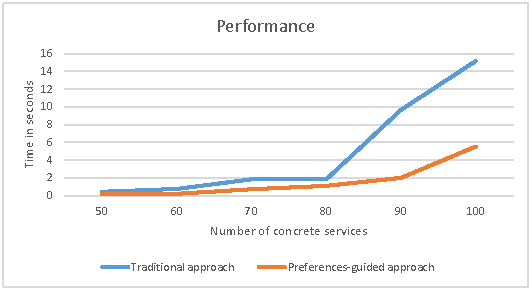
\includegraphics[scale=0.8]{fig1.pdf}
\caption{Performance evaluation.}\label{fig01}
\end{figure} 

The experiments include two different approaches: (i) the \textit{traditional approach} in which user preferences and SLAs are not considered; and (ii) the \textit{preference-guided approach} (P-GA) which considers the users' integration requirements and SLAs.

\begin{figure}[!h]
\centering
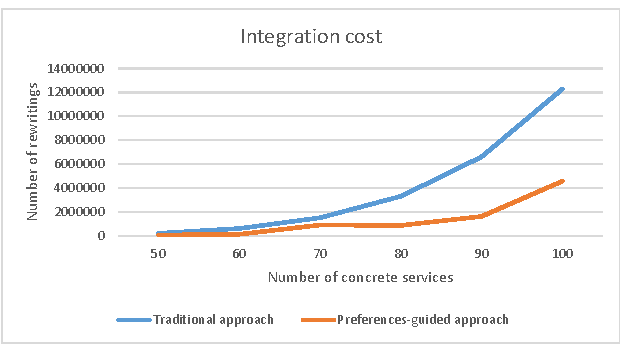
\includegraphics[scale=0.8]{fig2.pdf}
\caption{Performance evaluation.}\label{fig02}
\end{figure} 

The results P-GA are promisingly.  
The \textit{Rhone} increases performance reducing rewriting number which allows to go straightforward to the rewriting solutions that are satisfactory avoiding any further backtrack and thus reducing successful integration time (Figure~\ref{fig01}). Moreover, using the P-GA to meet the user preferences, the quality of the rewritings produced has been enhanced and the integration economic cost has considerable reduced while delivering the expected results (Figure~\ref{fig02}). However, the \textit{Rhone} still need to be tested in a large scale case and in a context of parallel multi-tenant to test efficacy.